\documentclass[14pt]{beamer}
\usepackage{beamerthemeshadow}
\usepackage{graphicx}
\usepackage{color, colortbl}
\usepackage[utf8]{inputenc}
\usepackage{hyperref}
\usepackage{makecell}                       %potrebno za formatiranje tabele
%\usepackage[flushleft]{threeparttable}     %ne koristimo ovo?

\usepackage[english, serbian]{babel}        %da ne bi pisalo "Table" nego "Tabela" i slično

\definecolor{electricpurple}{rgb}{0.75, 0.0, 1.0}
\definecolor{lightpurple}{rgb}{1.0, 0.75, 1.0}
\definecolor{lightpurple1}{rgb}{1.0, 0.92, 1.0}
\definecolor{lightpurple2}{rgb}{1.0, 0.97, 1.0}
\setbeamercolor{structure}{fg=electricpurple}

\def\d{{\fontencoding{T1}\selectfont\dj}}
\def\D{{\fontencoding{T1}\selectfont\DJ}}


\title{Analogni računari}
\subtitle{-- Tehničko i naučno pisanje --}
\author{Aleksandar Končalović, Veljko Josipović, Veljko Strugar, Uroš Janković}
\institute{Matematički fakultet\\Univerzitet u Beogradu}
\date{
	\footnotesize{Beograd, 2022.}	
}

\begin{document}
\begin{frame}
	\thispagestyle{empty}
	\titlepage
\end{frame}

\addtocounter{framenumber}{-1}

\section{Analogni Računari}
\begin{frame}[fragile]\frametitle{Istorija}
	\begin{itemize}
		\item Rani početak
		\begin{itemize}
			\item Prvi najraniji primer analognog računara jeste mehanizam sa Antikitere napravljen u Grčkoj i koristila se za računanje pozicija astronomskih tela.
		\end{itemize}
	\end{itemize}
\begin{itemize}
	\item Nakon mehanizma sa Antiketere
    \item Moderno doba
	\begin{itemize}
	\end{itemize}
 \begin{center}
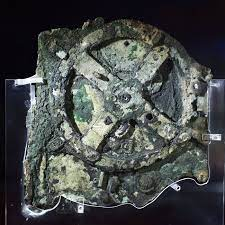
\includegraphics[scale=0.5]{MehanizamSaAntiketere.jpg}
\end{center}
\end{itemize}
\end{frame}


\begin{frame}[fragile]\frametitle{Princip rada analognih računara}
	\begin{itemize}	
		\item Obrađivanje kontinualnih veličina
		  \begin{itemize}
                \item Količina vode u cevima, intenzitet magnetne sile, vibracije tla kod seizmografa temperatura raznih supstanci...
            \end{itemize}          
	

\item Operacija sabiranja dva broja

\item Operacija množenja dva broja \\ $$ U = R*I $$
\end{itemize}
\begin{figure}[h!]
\begin{center}
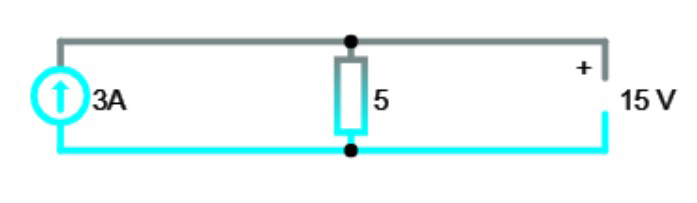
\includegraphics[scale=0.6]{Struja.jpg}
\end{center}
\caption{Vizuelni prikaz množenja}
\label{fig:h1}
\end{figure}
\end{frame}

\begin{frame}[fragile]\frametitle{Podela}
	\begin{itemize}
		\item Podela prema nameni
		\begin{itemize}
			\item Specijalne
            \item Univerzalne
            \item Kombinovane
		\end{itemize}
	\end{itemize}
\begin{itemize}
	\item Podela prema načinu dobijanja rešenja
	\begin{itemize}
		\item Spori
        \item Repetitivni
	\end{itemize}
\end{itemize}
\end{frame}

\begin{frame}{Primeri}
	\begin{itemize}
		\item Logaritmar
		\item Al-Jazarijev sat u zamku
 		\item Diferencijalni analizator
		\item Analogni analizator
		\item Analogni sat
	\end{itemize}
\end{frame}

\begin{frame}{Hidrointegrator Mike Alasa}
\begin{itemize}
    \item Najavio Ljubomir Klerić 1896.
    \item Završen 1899.
\end{itemize}
\begin{figure}[h!]
\begin{center}
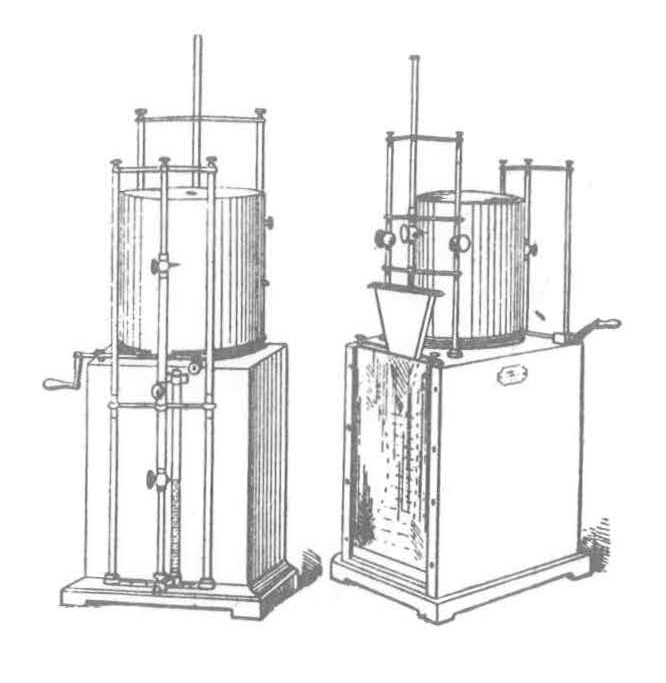
\includegraphics[scale=0.6]{h1.jpg}
\end{center}
\caption{Petrovićeva skica hidrointegratora. }
\label{fig:h1}
\end{figure}
    
\end{frame}

\begin{frame}[fragile]\frametitle{Elektronski analogni računari}
	\begin{itemize}
		\item Prednosti elektronskih analognih računara u odnosu na mehaničke:
		\begin{itemize}
			\item manja veličina
			\item lakša prenosivost
			\item niža cena
			\item  veća brzina
		\end{itemize}
	\end{itemize}
\begin{itemize}
	\item Helmut Helcer (nem. Helmut Hölzer) - prvi elektronski analogni rčunar
	\begin{itemize}
		\item operacioni pojačavač
		\item potenciometar koeficijenta
	\end{itemize}
\end{itemize}
\end{frame}

\section{Zaključak}
\begin{frame}[fragile]\frametitle{Zaključak}
	\begin{scriptsize}
	\begin{table}
		\caption{Prvi značajni elektronski analogni računari}
		\begin{tabular}{| c | c | c |}
			\hline
			\rowcolor{lightpurple}
			\textbf{Razvojni centar} & \textbf{Projekti} & \textbf{Datum} \\
			\hline
			\rowcolor{lightpurple1}
			Američka mornarica & \emph{Ciklon}, \emph{Tajfun}, MIT simulator letenja & 1946 - 1958 \\
			\rowcolor{lightpurple2}
			RAND korporacija & RAND analogni računar & 1948 \\
			\rowcolor{lightpurple1}
			Američka avijacija & GEDA / BEAC & 1950 \\
			\rowcolor{lightpurple2}
			RAE / Elliot Brothers ltd. &TRIDAC & 1950 - 1955 \\
			\rowcolor{lightpurple1}
			Engleska elektroindustrija & LACE & 1953 - 1956 \\ 
			\hline
		\end{tabular}
	\end{table}
	\end{scriptsize}

	\begin{itemize}
		\item Sažetak
		\begin{itemize}
			\item rade nad kontiaunalnim veličinama
			\item digitalni računari im nisu zamena (i jedni i drugi se simultano koriste)
			\item primena u astronomiji, matematici, vojnom i vazduhoplovnom inženjerstvu, elektrotehnici...
		\end{itemize}
	\end{itemize}
	
\end{frame}

\section{Literatura}

\begin{frame}[fragile]\frametitle{Literatura}
	\begin{itemize}	
		\scriptsize \item Jo Marchant, "Archimedes and the 2000-year-old computer" New Scientist, 12 December 2008.

\scriptsize \item E G Fischer (1912), "The Coast and Geodetic Survey Tide Predicting Machine No. 2".

\scriptsize \item Srpska akademija nauka i umetnosti, "Hidrointegrator Mihaila Petrovića Alasa". Pristupljeno 6.11.2022.

\scriptsize \item Thomas H. Lange. "Peenemuende, Analyse einer Technologieentwicklung im Dritten Reich". VDI-Verlag, Dusseldorf, 2006.
			
\scriptsize \item Bissell, C.C. (2004). "A great disappearing act: the electronic analogue computer". IEEE Conference on the History of Electronics, Bletchley, UK, 28-30 Jun 2004.
\end{itemize}
\end{frame}

\end{document}
